\begin{abstract}
We examined 111 studies, published from 2012 onward, that describe low-cost ultraviolet, visible, or near-infrared spectrophotometers, and traced how optical design, calibration, validation, cost, and openness vary across six hardware families. Just under half of these studies tested their instruments on samples that had not been used for calibration, a similar share reported how repeatable the readings were, and only about a quarter shared design files or code. Since the studies measured different targets, evaluated them in different ways, and counted costs differently, they cannot be used to rank the hardware families against one another. To complement the literature, we compared three instruments with a laboratory spectrophotometer under a single protocol: an AS7265x multispectral sensor (system A), a Raspberry Pi camera behind a pocket grating spectroscope (system B), and a commercial webcam grating spectrometer (system C). On three food-dye solutions kept out of calibration fitting and model selection, the root-mean-square absorbance differences over 400--700~nm were 0.281, 0.077, and 0.094, respectively. These figures describe the particular units and acquisition procedures we tested. We end with an application-dependent reporting checklist meant to help readers decide whether a low-cost instrument suits a given measurement, and to help others rebuild it.
\end{abstract}

\noindent\textbf{Keywords:} Low-cost spectrophotometry; Open-source instrumentation; Ultraviolet--visible spectroscopy; UV--Vis spectroscopy; Multispectral sensors; Absorbance calibration; Method validation; Reproducibility

\section{Introduction}\label{sec:intro}

Cheap optoelectronic parts and openly shared construction files have put spectrophotometry within reach of classrooms, small laboratories, and field teams.\citep{pereira2019low,laganovska2020portable,feng2021open} Building an instrument is no longer the hard part. The harder question is whether a particular instrument is good enough for the measurement it is supposed to make, and the published figures do not always settle it. Camera-based devices, for instance, can yield linear concentration calibrations even when their absorbance readings differ substantially from those of a laboratory spectrophotometer,\citep{grasse2015teaching,bruininks2022inexpensive} which is why a high calibration $R^2$ tells us little about how accurately new samples will be measured.\citep{prairie2020accurate,cirrone2026analytical}

Earlier reviews have dealt with parts of this field: smartphone spectrometers,\citep{mcgonigle2018smartphone} miniaturized near-infrared (NIR) instruments,\citep{bec2022miniaturized} chip-scale spectrometers,\citep{yang2021miniaturization} instruments for chemistry teaching,\citep{shidiq2020simple} and the validation of freshwater sensors.\citep{cirrone2026analytical} In this review we bring these strands together and ask how the way an instrument is built relates to what it has been shown to do, and to how easily someone else could reproduce it. We sort the instruments into six hardware families: light-emitting-diode (LED) photometers and colorimeters, smartphone grating spectrometers, camera grating spectrometers, integrated spectrometer modules, multispectral sensor chips, and a small group of other designs. To see how some of these issues play out in practice, we also measured three inexpensive instruments, which we refer to as systems A, B, and C, against a laboratory spectrophotometer using a common absorbance protocol. Both the literature and our own measurements then feed into a reporting checklist whose items depend on the intended application.

\subsection{Literature search and selection}\label{sec:method}

The review cites 138 documents (Figure~\ref{fig:sources}). Of these, 111 are device studies, and all counts and comparisons in the review are based on them; the remaining 27 are supporting documents. Among the supporting documents, 15 came from the literature search, seven are additional contextual or methodological references, and five are technical documents such as instrument specifications, a sensor datasheet, and software documentation.

We searched the literature in October 2026 by two routes. The first was a set of 18 OpenAlex queries restricted to publications from 1 January 2015 onward; keeping the first 50 results of each query yielded 789 unique records. The second route followed the reference lists of selected reviews and the works citing McGonigle et al., Geng et al., Cirrone et al., and Coppola et al.,\citep{mcgonigle2018smartphone,geng2017recent,cirrone2026analytical,coppola2024i} supplemented by nine targeted queries on multispectral chips, and yielded 1325 unique records. Because citation searching also reached older work, the corpus goes back to 2012.

We included English-language journal articles and full conference papers that describe low-cost ultraviolet (UV), visible, or NIR instruments for absorbance, transmittance, or reflectance measurements, including instruments built around commercial spectral modules. No price ceiling was imposed. An instrument counted as low cost when its authors described it that way and its construction was consistent with that description. As a result, reported totals range from about USD~1 to 1100 and cover quite different sets of equipment. Studies of individual components and radiometric characterizations served as supporting evidence on spectral response and stability.

We excluded fluorescence-only, Raman, laser-induced breakdown, and imaging-only instruments, as well as on-chip computational spectrometers, preprints, conference abstracts, and assays carried out only with commercial instruments. Cameras were eligible if they recorded spectra or if their images were synchronized with a separate point spectrum. These criteria defined the device corpus; the contextual engineering references played a supporting role only.

For every study we recorded the design, components, spectral capability, calibration, samples, reference comparisons, performance, cost, and availability of files. A characteristic was counted only if the study documented it explicitly. One author extracted the data and coded each study, and a second author checked the coding; disagreements were resolved by discussion. The queries, screening records, definitions, and source evidence are available from the authors on reasonable request.

\begin{figure}[!htbp]
\centering
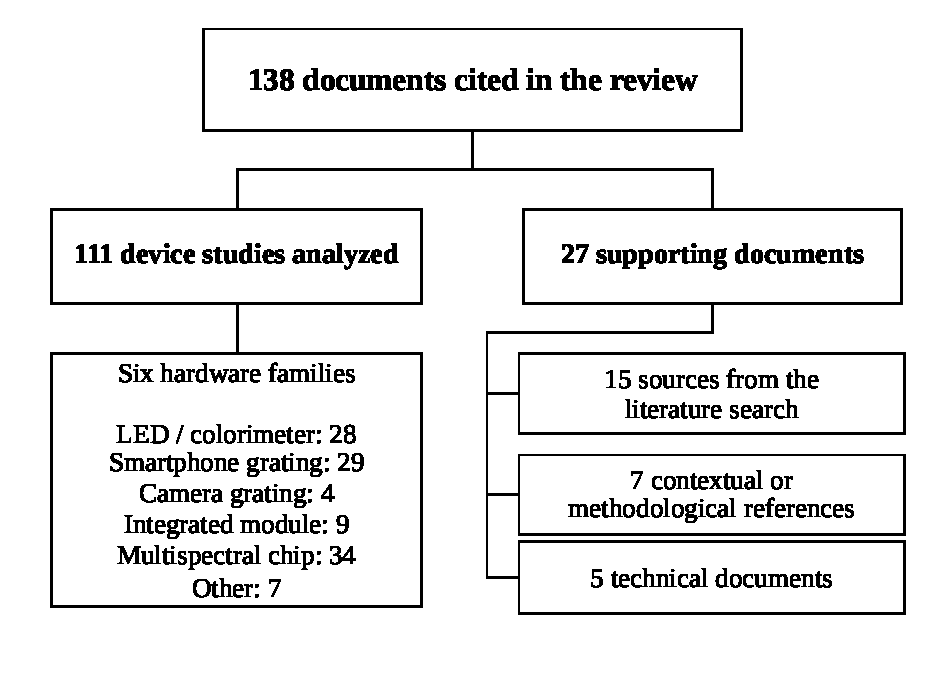
\includegraphics[width=\linewidth]{prisma.pdf}
\caption{\FigureCaptionOne}\label{fig:sources}
\end{figure}
\FloatBarrier
